\documentclass[11pt,a4paper]{article}
\usepackage[T1]{fontenc}
\usepackage{lmodern}
\usepackage{microtype}
\usepackage[margin=27mm,headheight=15pt]{geometry}
\usepackage{amsmath,amssymb,amsthm,mathtools}
\usepackage{booktabs,longtable,array,enumitem,graphicx,xcolor}
\usepackage{fancyhdr,hyperref,cleveref}
\usepackage[most]{tcolorbox}
\definecolor{navy}{HTML}{17324D}
\definecolor{teal}{HTML}{087E8B}
\definecolor{paperblue}{HTML}{EFF5FA}
\hypersetup{colorlinks=true,linkcolor=navy,citecolor=teal,urlcolor=teal,
  pdftitle={Component Disc Certificates and Quadrilateral Core Reduction},
  pdfauthor={ProveIt research continuation}}
\pagestyle{fancy}
\fancyhf{}
\fancyhead[L]{\small\textcolor{navy}{ProveIt / Unknot recognition}}
\fancyhead[R]{\small October 2026}
\fancyfoot[C]{\thepage}
\renewcommand{\headrulewidth}{0.3pt}
\setlist{itemsep=3pt,topsep=5pt}
\newtheorem{theorem}{Theorem}[section]
\newtheorem{lemma}[theorem]{Lemma}
\newtheorem{proposition}[theorem]{Proposition}
\newtheorem{corollary}[theorem]{Corollary}
\theoremstyle{definition}
\newtheorem{definition}[theorem]{Definition}
\newtheorem{example}[theorem]{Example}
\theoremstyle{remark}
\newtheorem{remark}[theorem]{Remark}
\newcommand{\Z}{\mathbb Z}
\newcommand{\F}{\mathbb F}
\newcommand{\D}{\mathcal D}
\newcommand{\poly}{\operatorname{poly}}
\newcommand{\bits}{\operatorname{bits}}
\newcommand{\supp}{\operatorname{supp}}
\newcommand{\code}[1]{\texttt{\detokenize{#1}}}
\newcommand{\baseline}{\texttt{7518823550fb}}
\newtcolorbox{resultbox}{colback=paperblue,colframe=navy,boxrule=0.5pt,
  arc=1pt,left=9pt,right=9pt,top=8pt,bottom=8pt}
\title{\textcolor{navy}{Toward Quasi-Polynomial Unknot Recognition}\\[5pt]
  \large Component Disc Certificates and Quadrilateral Core Reduction}
\author{Research continuation for Vladimir Reshetnikov's ProveIt project}
\date{9 October 2026\\\small Source snapshot and computations: 9 October 2026 UTC}
\begin{document}
\maketitle
\begin{abstract}
The maintained normal-surface backend computes aggregate component counts but
does not decide whether a disconnected supplied surface contains a compressing
disc. We implement and certify this missing operation without expanding binary
normal coordinates. The main specialization uses only three additive orbit
weights: Euler characteristic and two boundary-homology tests. A second
reduction removes vertex-link components and divides by the content of the
quadrilateral coordinates. We prove that the exact number of essential disc
components scales linearly under this reduction, although the total number of
surface components need not. The resulting orbit query depends on the bit size
of the primitive quadrilateral data, independently of large additive triangle
offsets. Independent arithmetic replay, explicit finite oracles, external
Regina comparisons, and paired measurements accompany the implementation.
A further proved two-weight variant uses certified ambient homology
preprocessing; its implementation and timing are future work.
The work is an algorithmic continuation of classical weighted
Agol--Hass--Thurston counting and normal-surface Q-theory. It does not establish
a general quasi-polynomial unknot recognizer: candidate generation, certified
diagram-to-exterior provenance, and the accelerated hierarchy remain separate
obligations.
\end{abstract}
\vspace{3pt}
\begin{resultbox}
\textbf{Scope of the proved result.}
Given a validated finite triangulation with one torus boundary and an admissible
binary normal vector, the delivered procedure counts its compressing-disc
components in polynomial time in the encoded input. It can certify a positive
count even when the surface is disconnected and its total boundary class is
zero. A zero count concerns that vector alone.
\end{resultbox}
{\small\tableofcontents}
\clearpage
\section{Result, scope, and relation to the repository}\label{sec:results}

\subsection{The concrete problem addressed}

Let $\mathcal T$ be a finite triangulation of a compact connected orientable
three-manifold whose boundary is one torus. Let $x\in\Z_{\geq0}^{7t}$ be an
admissible normal vector, where $t$ is the number of tetrahedra. Write $S(x)$
for the corresponding embedded normal surface. The input coordinates are
binary integers; neither $S(x)$ nor its components are supplied as expanded
cell complexes. Define
\[
  \D(x)=\#\{C\in\pi_0(S(x)):C\text{ is a disc with essential boundary}\}.
\]
All multiplicities in this definition count actual components. In particular,
$10^{100}$ parallel meridian discs contribute $10^{100}$, not one.

The previous native backend obtains the number of components, orientability
counts, boundary-curve count, and total Euler characteristic through interval
orbits, with optional additional classification of closed and boundary-touching
components. Its positive disc predicate requires the \emph{whole supplied
surface} to be connected. The maintained boundary-classification discussion
explicitly leaves componentwise disc identification unresolved
\cite{ProveItSnapshot}. The new operation computes $\D(x)$ for a disconnected
surface and supplies replayable evidence for the answer.

This is a sharply delimited algorithmic improvement. A positive answer proves
that the supplied manifold has compressible boundary. If that manifold has
independently been identified with the exterior of an input knot in $S^3$, it
certifies unknottedness. A zero answer only eliminates this particular vector.
It does not eliminate other normal surfaces, prove boundary incompressibility,
or establish knottedness. The delivered code does not silently add any of
these missing implications.

\subsection{Main statements}

\begin{theorem}[Three-weight disc query]\label{thm:main-disc}
For the validated input class above, there is an algorithm that computes
$\D(x)$ and a compressed histogram of componentwise Euler characteristic and
boundary homology using three integer weights per orbit representative.
Its running time, output length, and certificate length are polynomial in
$t$ and the maximum input-coordinate bit length. Its certificate can be
checked without invoking its orbit-discovery scheduler or its weight-transport
implementation.
\end{theorem}

The topology in this theorem is proved in \cref{sec:geometry}; the compressed
algorithm and its bit accounting are established in \cref{sec:weighted-orbits}.
The checker shares the finite-manifold input validator and the deterministic
cell-weight construction. Independence therefore concerns discovery and
arithmetic transport, not two unrelated implementations of the entire
topological input model.
A further refinement to two weights after certified ambient homology
preprocessing is proved in \cref{sec:two-weight-refinement}. That variant is
not implemented or included in the reported timings.

\begin{theorem}[Primitive quadrilateral core]\label{thm:main-core}
For each global vertex $v$, let $\ell_v$ be the least triangle coordinate
among the tetrahedral corners at $v$, and let $L_v$ be its vertex-link vector.
If $x$ has a nonzero quadrilateral coordinate, let $g$ be the gcd of its
quadrilateral coordinates and set
\[
 P=\frac{x-\sum_v\ell_v L_v}{g},\qquad
 Q=\max_j\frac{x_{q_j}}{g}.
\]
Then $P$ is an admissible nonnegative integral normal vector and
\[
                  \D(x)=g\D(P).
\]
Every coordinate of $P$ is at most $\max(1,4t-1)Q$. If all quadrilateral
coordinates vanish, $\D(x)=0$ and no orbit computation is needed.
\end{theorem}

The full proof, including the effect of one-sided components under scaling,
appears in \cref{sec:quadrilateral-core}. The central computational consequence is that
the expensive orbit query can use
\[
                    O(\log(t+1)+\log(Q+1))
\]
bits per geometric coordinate. Large common multiplicity and large independent
vertex-link offsets still have to be read and processed, but they disappear
from the subsequent orbit search. This remains useful when the gcd of the
\emph{original seven-coordinate vector} is one.

\subsection{Which parts are established antecedents?}

The weighted orbit method and polynomial component recovery are classical
Agol--Hass--Thurston results. Canonical removal of vertex links and conversion
between quadrilateral and standard coordinates are classical Q-theory.
We use them openly rather than describe them as new topology
\cite{AHT2006,Tollefson1998,Burton2009}. The contribution here is the implemented
specialization, its source-bound certificate, its exact disc-count reduction,
and its measured improvement against more expensive routes to the same query.
We do not claim that the specialized mathematical statements have no earlier
appearance in the literature.

\begin{center}
\begin{tabular}{>{\raggedright\arraybackslash}p{0.30\linewidth}>{\raggedright\arraybackslash}p{0.59\linewidth}}
\toprule
Ingredient & Status in this continuation \\
\midrule
Weighted interval orbits & Classical algorithm; newly implemented as a
checked extension of the maintained repository trace. \\
Vertex-link canonicalization & Classical construction, used with explicit
binary-cost and quadrilateral-content accounting. \\
Three statistics for disc detection & A proved specialization that avoids
recovering $7t$ weights or counting orientation and boundary covers. \\
Two weights with ambient homology & Proved refinement; implementation and
performance comparison remain future work. \\
Disconnected disc census & New native repository capability with finite
oracles and source-bound replay. \\
General quasi-polynomial recognition & Remains unimplemented and unproved
for the delivered pipeline. \\
\bottomrule
\end{tabular}
\end{center}

\subsection{Why aggregate invariants are insufficient}

There are two different pitfalls. First, even parallel meridian discs have
zero \emph{total} mod-two boundary class. Thus requiring a nonzero total
class rejects valid positive examples. Second, a surface can have total
Euler characteristic one and a nonzero total boundary class without containing
a disc. For example, a small interior vertex-link sphere disjoint from an
orientable genus-one spanning surface has total Euler characteristic
$2+(-1)=1$. The sphere has no boundary and the genus-one component is not a
disc. The corresponding finite normal-surface example is included in the
external audit.

The new query associates Euler characteristic and boundary class to the
\emph{same connected component}. Its correctness does not follow from a
test of the sums of these quantities. This distinction is the main reason
weighted orbits are needed.

\subsection{Exact API contracts}

The new APIs are additive modules under \code{fastunknot}; existing recognizer
defaults, certificate versions, and old aggregate APIs are unchanged. The
following table specifies the information computed by each route.

\begin{center}
\begin{tabular}{>{\raggedright\arraybackslash}p{0.29\linewidth}>{\raggedright\arraybackslash}p{0.12\linewidth}>{\raggedright\arraybackslash}p{0.47\linewidth}}
\toprule
Route & Dimension & Certified output \\
\midrule
\code{mode='disk'} & $3$ & Component histogram of $(\chi,h_1,h_2\bmod2)$,
total components, and essential-disc count. \\
\code{mode='summary'} & $5$ & The preceding data, normal-disc count, and
boundary intersection weight for each histogram type. \\
\code{mode='coordinates'} & $7t$ & Actual connected-component normal vectors,
grouped with binary multiplicities, and their disc predicates. \\
Reduced count API & $3$ on $P$ & Essential-disc count of the original $x$,
with a certified canonical reduction. \\
\bottomrule
\end{tabular}
\end{center}

Boundary intersection weight is the number of normal boundary edge points,
equal to the number of boundary normal arcs. It is \emph{not} the number of
boundary circles. The reduced count API intentionally makes no claim about
the total number of original components: that quantity is not homogeneous
in the presence of one-sided components. The full-coordinate route can
extract a concrete disc vector for a later cutting operation, but finding
and certifying that cut is outside this package.

\subsection{The quasi-polynomial target in the inspected sources}

The explicit March 2021 slides announce
$2^{O((\log n)^3)}=n^{O((\log n)^2)}$ time; the institutional announcement
instead uses $n^{c\log n}$. Both are quasi-polynomial, but the exponents are
different \cite{LackenbySlides,Oxford2021}. The July 2026 preprint provides a
hierarchy algorithm and polynomial verification results, while separating
iteration counts from step costs that have not all been specified sufficiently
for runtime analysis \cite{Lackenby2026}. The repository makes the same
distinction. Consequently this article treats quasi-polynomial time as the
global implementation target and states the local proved bounds explicitly.

The selected source snapshot is commit \baseline, whose full identity is
recorded in the provenance manifest. This pins the comparison despite active
development elsewhere in the repository. No remote repository changes are
required to inspect, reproduce, or integrate the accompanying archive.

\section{Weighted interval orbits with polynomial output}
\label{sec:weighted-orbits}

Weighted orbit counting is classical. Agol, Hass, and Thurston prove a
polynomial-time weighted extension of their interval algorithm in Theorem~16;
their Corollary~17 applies it to the normal coordinates of connected surface
components \cite{AHT2006}. We use this antecedent explicitly. The contribution
here is a maintained implementation with a precise suffix-transport invariant,
a compressed histogram contract, independently checked arithmetic, and the
small set of weights needed by the subsequent disc query. Neither weighted
counting itself nor the deduction that normal components can be recovered in
polynomial time is claimed as new.

\subsection{Input, output, and the surviving-representative invariant}

Let $X=\{0,\ldots,N-1\}$, with an equivalence relation generated by $K$
interval pairings. Each pairing is an isometry between equal-length integer
intervals, with either sign. Endpoints and $N$ are binary integers. A weight
function $w:X\to\Z^d$ is supplied by $s$ additive half-open intervals:
\[
 w(x)=\sum_{i=1}^{s} v_i\,\mathbf 1_{[\ell_i,r_i)}(x),
 \qquad v_i\in\Z^d.
\]
Intervals may overlap, coordinates may be negative, and uncovered points have
zero weight. Sorting their endpoints and summing differences produces a
canonical list of constant runs covering $X$. Adjacent equal runs are merged.
For $N>0$ the initial number $R_0$ of runs is at most $2s+1$; the empty universe
has no runs.

For an orbit $O$, define $W(O)=\sum_{x\in O}w(x)$. The output is the sorted
histogram
\[
 H(v)=\#\{O:W(O)=v\}, \qquad H(v)>0
\]
on its explicitly represented support. Multiplicities remain binary integers.
The algorithm does not emit one record per orbit. For example, an unpaired
universe of size $2^b$ with constant weight $v$ has the one-record answer
$H(v)=2^b$. Expanding that answer into a list would destroy the claimed encoded
complexity. Distinct components with the same weight deliberately share a
record; their identities and attaching maps are not part of this contract.

The unweighted producer supplies a complete AHT reduction trace. It contains
identity deletion, reflection trimming, periodic merging, transmission,
static-interval contraction, and suffix truncation. Both the classical and
Fine--Wilf merger versions are supported by the existing independent trace
checker. Weight propagation reconstructs the current pairing list from these
events, without running the discovery scheduler again.

The relevant invariant is stronger than conservation of the total weight.
Each surviving point represents a disjoint collection of original points;
its current weight is their vector sum. The current orbit relation groups
these collections into exactly the original orbits not yet emitted. Identity
deletion, trimming, merging, and transmission change the generators of the
relation without removing points. They therefore leave all point weights
unchanged. Only the two point-removal operations require weight updates.

\subsection{Exact transport through a truncation}

Suppose the current universe is $[0,N)$ and a checked event removes the suffix
$[c,N)$. That suffix is incident only to its designated carrier pairing.
For a translation carrier with displacement $p>0$, its domain begins at $a$,
its range begins at $a+p$, and $c\ge a+p$. Repeated inverse application sends
every deleted point to the retained interval $J=[c-p,c)$ by
\begin{equation}
 f(x)=c-p+\bigl((x-(c-p))\bmod p\bigr).
 \label{eq:weighted-residue-map}
\end{equation}
All intermediate inverse applications are defined: until the first value
below $c$, the point remains in the carrier's range. The target belongs to
$[a,c)$ and is retained. Each original orbit still has a representative.

Consider one constant suffix run $[\ell,r)$ of value $v$. Write
\[
 r-\ell=qp+u,\qquad 0\le u<p,
 \qquad z=c-p+((\ell-(c-p))\bmod p).
\]
Its pushforward contributes $qv$ to every point of $J$. The remaining $u$
points contribute $v$ on the cyclic interval of length $u$ starting at $z$.
Putting $u_1=\min(u,c-z)$, this is the sum of contributions on
\[
 [z,z+u_1),\qquad [c-p,c-p+u-u_1).
\]
Empty intervals are omitted. Thus a run of astronomical length needs one
division with remainder and at most three constant-interval additions. The
retained prefix keeps its existing weights, and all suffix contributions
are added to it using an endpoint-difference table.

A checked reflection carrier has disjoint domain and range after trimming.
With current right endpoint $N-1$ and left endpoint $a$, its inverse is
$x\mapsto a+N-1-x$. Consequently a deleted run $[\ell,r)$ maps bijectively to
\[
 [a+N-r,a+N-\ell).
\]
This interval lies wholly in the retained prefix. The implementation adds
the same vector there and discards the source suffix. The reflection's
order reversal must be retained; treating every pairing as a translation
would give incorrect component sums even when the unweighted count agreed.

For a static contraction, every point in each supplied gap is a singleton
orbit of the current relation. Its accumulated weight is already the full
weight of one original orbit. Intersecting the gaps with the current runs
therefore adds the intersection lengths to the corresponding histogram
entries. The remaining points and weights are shifted by the same
order-preserving gap-removal map used for the pairings.

\begin{proposition}[Correct weighted replay]
\label{prop:weighted-correct}
Replaying these operations along a valid complete AHT trace returns exactly
the histogram of original orbit-weight sums, including signed weights.
\end{proposition}
\begin{proof}
Maintain the disjoint representative collections described above. The four
relation-only operations preserve them unchanged. A suffix truncation assigns
each deleted collection to its image under the carrier's inverse, possibly
iterated. These assignments partition all deleted collections and preserve
their original orbit membership. Summing their vectors gives exactly the
displayed pushforward formulas. A static point then represents one complete
original orbit and can be emitted. The checked trace finishes with no points
and no pairings, so every original orbit is emitted exactly once. No step uses
positivity; the proof applies coordinatewise in the additive group $\Z^d$.
\end{proof}

\subsection{A bound on run growth and histogram size}

The fact that one source run gives constantly many intervals is insufficient
to prove polynomial space: repeated constant-factor growth could still be
exponential. The necessary bound follows from transporting jumps.

\begin{lemma}[Additive run growth]
\label{lem:weighted-run-growth}
A truncation increases the number of canonical weight runs by at most two.
A static contraction does not increase it. Thus after $E$ trace events,
\[
 R\le R_*:=R_0+2E.
\]
\end{lemma}
\begin{proof}
Split the old runs at the truncation point into $P$ nonempty prefix runs and
$Q$ nonempty suffix runs. At most one old run was split, so
$P+Q\le R+1$. Extend the suffix function by zero to the integer line. Its
discrete derivative has jumps only at its $Q+1$ endpoints. Under translation
folding, each jump has one residue image modulo $p$. The cutoff endpoint
maps to the wrap boundary $c-p$, leaving at most $Q$ other interior residue
locations. Relative to the $P-1$ internal prefix boundaries, these locations
and the possible new wrap boundary give at most $P+Q+1$ runs. This is at most
$R+2$. Coincident endpoints and cancelling jumps only reduce the count.

For a reflection, the $Q+1$ suffix endpoints have one reflected image each.
Together with the $P-1$ prefix boundaries they again give at most
$P+Q+1\le R+2$ runs. Finally, deleting static intervals retains a subsequence
of the old constant runs. Every new change of value corresponds to at least
one old change between consecutive retained points. Coalescing adjacent equal
values therefore cannot increase the run count.
\end{proof}

If a contraction contains $g$ gaps, their intersections with a run list have
at most $R+g-1$ nonempty pieces. There are at most $2K+1$ gaps, since all
pairing domains and ranges together have at most $2K$ occupied intervals.
Pairing count never increases during the trace. Consequently the number $h$
of distinct histogram records satisfies the conservative bound
\begin{equation}
 h\le E\bigl(R_0+2E+2K+1\bigr).
 \label{eq:weighted-output-bound}
\end{equation}
Repeated equal weights share a record, so this bounds the actual output as
well as the number of possible emissions. Since the maintained AHT trace
length is polynomial in $K$ and $\log(N+1)$, the histogram has polynomial
encoded size. This observation is essential when the number of components
itself is exponentially large.

\subsection{Arithmetic and certificate complexity}

Assume every coordinate of every supplied $v_i$ has absolute value at most
$A$. Each current representative contains a subset of original points, hence
every accumulated coordinate has magnitude at most $NsA$. This also bounds
each completed orbit sum. Taking
\[
 B=O\bigl(1+\log(N+1)+\log(s+1)+\log(A+1)\bigr)
\]
therefore bounds all weight bit lengths. Multiplicities use
$O(1+\log(N+1))$ bits. Quotient multiplication is integer multiplication on
these bit lengths, not a unit-cost operation on arbitrarily large numbers.

Initial normalization uses $O(sd)$ coordinate additions and $O(s\log(s+1))$
endpoint comparisons. Given a trace of $E$ events, one truncation uses
$O(dR_*)$ coordinate operations and $O(R_*\log(R_*+1))$ endpoint comparisons.
A contraction requires at most
$O(d(R_*+K)+(R_*+K)\log(R_*+K+1))$ such operations. Source reconstruction and
the final histogram sort add polynomial costs; lexicographic sorting of $h$
vectors uses at most $O(dh\log(h+1))$ coordinate comparisons. A useful
event-sensitive accounting bound, apart from the existing unweighted
producer and checker, is therefore
\[
 O\!\left(sd+s\log(s+1)
 +E\bigl[d(R_*+K)+(R_*+K)\log(R_*+K+1)+K^2\bigr]
 +dh\log(h+1)\right).
\]
The $K^2$ term charges the independent weighted checker's direct reconstruction of contracted pairing endpoints across up to $O(K)$ gaps. The producer can use the sharper bound without that term. This counts arithmetic and ordinary dictionary operations. Integer hashing,
comparisons, additions, and products must then be charged their bit costs.
Adversarial collisions in Python dictionaries can worsen the displayed
container-operation model, but still give a polynomial bound for these
explicit polynomial-size tables; deterministic balanced maps give the usual
additional logarithmic alternative. No conclusion depends on treating a
$2^b$-bit integer as one machine word.

The certificate stores the canonical source weights, the existing unweighted
orbit proof, and the claimed sorted histogram. A contraction event can list
$O(K)$ gaps, so trace payload size is charged as well as event count. The run
bound, output bound, and bit bound together show polynomial certificate
length. Internally the producer creates an orbit trace even when the caller
does not request a returned certificate: weight propagation needs that
sequence of contractions. A supplied trace can instead be source-checked and
reused, avoiding a new orbit search.

\subsection{Independent arithmetic and sufficient statistics}

The independent weighted checker first verifies all unweighted local rules
against the caller's pairing list. It then reconstructs the pairing updates
and weight transport separately. In particular, its translation arithmetic
does not reuse the producer's quotient-and-remainder interval additions.
For the zero-extended suffix function $v$ and a target representative $y$, put
\[
 S(y)=\sum_{k\in\Z}v(y+kp).
\]
At the leftmost residue $y=c-p$, a source run $[\ell,r)$ contributes its
weight multiplied by
\[
 \left\lfloor\frac{r-1-y}{p}\right\rfloor
 -\left\lfloor\frac{\ell-1-y}{p}\right\rfloor.
\]
This determines one anchor value. The identity
\[
 S(y)-S(y-1)=\sum_{k\in\Z}\bigl(v(y+kp)-v(y-1+kp)\bigr)
\]
determines every remaining value by integrating the independently mapped
suffix jumps. These two arithmetic constructions reach the same required
pushforward through different calculations. The checker additionally checks
the total orbit count, exact sorted histogram, source binding, and signed
mass conservation. A partial histogram is never returned when the
underlying orbit allowance is exhausted; cancellation callbacks propagate
through construction and replay.

Finally, many decisions depend on a small additive signature rather than a
full component description. If an orbit predicate factors through $d_0$
additive statistics, those statistics may be transported directly and the
desired count obtained by summing histogram multiplicities satisfying the
predicate. The number of vector coordinates in the arithmetic bound becomes
$d_0$. In the next section, three statistics suffice for the disc predicate,
whereas full normal-component extraction uses $7t$ coordinates. This removes
a factor of order $t$ from the dimension-dependent arithmetic bound; it does
not remove common orbit-search and endpoint-processing costs. The signatures
also need not recover the normal vector of a particular disc. A subsequent
operation that actually cuts along a selected component can request the
full-coordinate mode and pay for its richer output.

\section{Cell weights and three-statistic disc detection}\label{sec:geometry}

\subsection{Validated finite geometry}

The existing validator checks reciprocal face pairings, face-connectedness,
ambient orientability, absence of reversed edge identifications, spherical
or disc vertex links, and a single finite boundary torus. Ideal vertices and
other boundary topologies are rejected. Normal coordinates are checked for
nonnegativity, face matching, and the quadrilateral constraints. These checks
are retained before any new component query.

The proof requires no irreducibility hypothesis on the supplied manifold.
Irreducibility becomes relevant to other recognition and hierarchy operations,
not to the classification of its embedded surface components. In particular,
the implementation must correctly reject a closed projective-plane component
as a disc even though its Euler characteristic is one.

For every global triangulation edge $e$, let $w_e$ be its normal intersection
number. A block of $w_e$ consecutive integers represents those intersection
points, ordered using a consistent orientation of that edge. Concatenate
these blocks to obtain a universe of size
\[
                        N=\sum_e w_e.
\]
Each normal arc in a face pairs its two endpoint positions. Consecutive arcs
of a fixed type give one interval isometry. Count a glued face once and each
boundary face once. The number of pairings is at most $12t$. The graph formed
by these vertices and arc edges is the one-skeleton of the normal surface's
polygonal cellulation. Its connected components are exactly those of the
surface. Identifications within one tetrahedron, loop arcs, and multiple
edges cause no problem for either connectivity or the Euler formula.

\subsection{Integral ownership of Euler characteristic}

One can distribute fractional Euler weights over polygon corners. We instead
use an integral ownership rule, which avoids denominators entirely.
Give every edge-intersection point an initial Euler weight $+1$. For every
normal arc, charge $-1$ to one of its endpoints. For every normal polygon,
charge $+1$ to one selected corner. The selected corner belongs to the same
surface component as the entire polygon; likewise the endpoint of an arc.
Therefore, for every component $C$,
\[
             \sum_{p\in C} w_\chi(p)=V(C)-E(C)+F(C)=\chi(C).
\]
This is true even when several selected local corners become the same global
intersection point: their additive contributions must then accumulate there.

All ownership data is described by $O(t)$ intervals. The negative arc charge
is assigned on the canonical source interval of each maintained pairing.
For a triangle type at vertex $v$, choose a fixed incident local edge and use
the triangle points nearest $v$. For an active quadrilateral type, choose the
lexicographically first local edge that it crosses. Along an edge from local
vertex $a$ to local vertex $b$, the points appear as triangles at $a$, then
quadrilaterals, then triangles at $b$. If their relevant counts are $T_a,Q$,
the selected quadrilateral corners occupy
\[
                            [T_a,T_a+Q).
\]
Reflect this interval if the local edge direction disagrees with the global
orientation. No stack is expanded.

\begin{lemma}[Cell-weight identity]\label{lem:cell-weight}
The constructed piecewise-constant integer weight has component sums
$\chi(C)$, and has an $O(t)$-interval additive description. A second weight
obtained by retaining just the polygon credits sums to the number of normal
polygons in $C$.
\end{lemma}
\begin{proof}
Every cell receives exactly one charge of its appropriate sign and each
charge lies in its own connected component. A tetrahedron has at most five
nonempty polygon types, and a face has at most three arc types. The listed
charges are constant on each type's consecutive set of corners or endpoints.
\end{proof}

The full-coordinate reference replaces each polygon credit by the corresponding
standard basis vector of $\Z^{7t}$. A component's orbit sum is then its actual
normal coordinate vector. This is the classical component-recovery route
\cite{AHT2006}; the new disc query avoids its growing vector dimension.

\subsection{A small, certified homology basis of the boundary}

Let $G$ be the primal one-skeleton of the boundary triangulation. Self-loops
and multiple edges are permitted. Select a spanning tree $T$ of $G$. In the
dual graph select a spanning tree $T^*$ using edges whose primal edges are
outside $T$. Exactly two primal edges are in neither tree, since the boundary
is a torus and
\[
 |E|-(|V|-1)-(|F|-1)=2.
\]
For each leftover edge, append the unique path in $T$ connecting its endpoints.
These two fundamental cycles, $c_1,c_2$, form a basis of
$H_1(\partial\mathcal T;\F_2)$.

For completeness, the tree-cotree fact can be seen by contracting the primal
tree and removing edges dual to a dual spanning tree. These operations
preserve the surface and reduce its cellular description to one vertex,
one face, and two edges. Over $\F_2$, the boundary of that face is zero,
and the two surviving cycles freely generate the two-dimensional first
homology. Reversing the contractions gives exactly the chosen fundamental
cycles. The dual graph outside the primal tree is connected: a separating
dual cut would correspond to a nonempty primal cycle contained in the tree.

The certificate checker does not rely on the spanning-tree algorithm's output
being correct. It independently checks that each proposed cycle has even
incidence at every vertex, constructs the boundary vectors of all triangles,
and performs binary Gaussian elimination. The two proposed cycles must each
increase the rank modulo the face-boundary span. Since the validator has
already established a torus, two independent classes are a basis. Repeated
edges of a triangular face cancel modulo two in this check.

\subsection{Boundary intersection weights}

For each $j\in\{1,2\}$, give every intersection point on a boundary edge in
$c_j$ a homology weight $+1$ in coordinate $j$; give every other point weight
zero. If $z_e(C)$ counts the boundary points of component $C$ on edge $e$, then
its orbit sum is
\[
                    \eta_j(C)=\sum_{e\in c_j} z_e(C).
\]
The code retains this as an exact integer and reduces it modulo two when
interpreting the result. Equivalently, one could carry an $\F_2$ coordinate
throughout the weighted algorithm; the present implementation uses one
uniform integer-vector engine for all query modes.

The parity vector $z_e(C)\bmod2$ is the cellular cocycle Poincare-dual to
$\partial C$: every boundary triangle meets the normal boundary curve in
arcs and therefore has even total endpoint incidence. Evaluating that cocycle
on the two basis cycles yields
\[
    h(C)=(\eta_1(C),\eta_2(C))\bmod2,
    \qquad
    h(C)=0\ \Longleftrightarrow\ [\partial C]=0
       \text{ in }H_1(\partial\mathcal T;\F_2).
\]
The equivalence uses the nondegenerate homology-cohomology pairing over the
field $\F_2$. It applies to the total boundary of each component, rather than
to one arbitrarily selected boundary circle.

\subsection{Three additive weights characterize compressing discs exactly}
\label{sec:three-weight-criterion}

Let $C$ be a connected component of the supplied proper normal surface.
The cell-incidence weight gives $\chi(C)$. Let $\gamma_1,\gamma_2$ be the
checked homology basis of the boundary torus described above, and define
\[
 h_i(C)=\sum_{e\in\gamma_i}|C\cap e|\pmod2,
 \qquad i=1,2.
\]
The raw orbit calculation retains the corresponding integer sums; parity is
taken only when interpreting the resulting component signature. In
particular, signed Euler arithmetic and binary homology arithmetic are not
silently identified.

\begin{lemma}
\label{lem:boundary-character-completeness}
The pair $(h_1(C),h_2(C))$ vanishes exactly when the mod-two boundary class of
$C$ vanishes in the ambient torus.
\end{lemma}
\begin{proof}
On every boundary triangle, a normal arc contributes two endpoints.
Consequently the parity of edge intersections is a cellular $1$-cocycle,
including in generalized triangulations where repeated face edges must be
combined modulo two. This cocycle represents the Poincar\'e dual of the
boundary multicurve. Evaluation on a homology basis determines its cohomology
class, since evaluation gives the nondegenerate pairing between
$H^1(T^2;\F_2)$ and $H_1(T^2;\F_2)$. Both spaces have dimension two. Thus
the two values vanish precisely for the zero boundary class.
\end{proof}

\begin{theorem}[Exact three-weight disc criterion]
\label{thm:three-weight-disc}
A connected component $C$ is a compressing disc for the ambient boundary
torus if and only if
\[
 \chi(C)=1,
 \qquad (h_1(C),h_2(C))\ne(0,0).
\]
\end{theorem}
\begin{proof}
A compressing disc has Euler characteristic one. Its boundary is an embedded
essential circle on the torus. Such a circle represents a primitive integral
slope, so its reduction modulo two is nonzero. The lemma proves necessity.

Conversely, the nonzero boundary class implies that $C$ has boundary. The
classification of connected compact surfaces now leaves only a disc. Indeed,
an orientable surface of genus $a$ with $b\ge1$ boundary circles has
$\chi=2-2a-b$; equality to one forces $a=0,b=1$. A nonorientable surface with
$k\ge1$ crosscaps and $b\ge1$ boundary circles has
$\chi=2-k-b\le0$. The resulting disc has nonzero boundary class, and hence
its simple boundary circle is essential on the torus.
\end{proof}

The boundary condition in this argument is necessary. A closed projective
plane also has Euler characteristic one; its two boundary evaluations are
zero, so it is correctly excluded. Such closed one-sided surfaces occur in
the supported general torus-boundary manifold fixtures, even though those
fixtures need not be knot exteriors. No assumption of irreducibility is
smuggled into the local component test.

Two binary linear probes are also the minimum needed to recognize the zero
element of the full torus boundary-class space by linear evaluation alone.
A single linear functional on the two-dimensional space has a nonzero
kernel. The two-probe statement concerns this unrestricted homology interface;
it does not prove a lower bound for a specially restricted collection of
normal surfaces in one fixed manifold, nor for nonlinear preprocessing.
Together with the Euler coordinate, it explains the natural three-weight
implementation and its reduction from $7t$-dimensional coordinate extraction.

The torus hypothesis cannot be dropped from the equivalence. On a boundary
surface of genus at least two, an essential separating simple circle can have
zero mod-two homology. The same predicate would then give only a sufficient
test for certain compressing discs, and could miss others. The native input
validator's one-torus-boundary contract is therefore part of the theorem,
not merely a convenience for constructing a small basis.

Finally, the test must be applied to individual component weights. Two
parallel meridians have zero total boundary class but contribute two
compressing discs. Conversely, an inessential vertex-link disc together with
a M\"obius band can have total Euler characteristic one and nonzero total
boundary class while contributing no compressing disc. A weighted orbit
histogram resolves both ambiguities without listing the components one by one.

\subsection{A proved two-weight refinement using ambient homology}
\label{sec:two-weight-refinement}

The three-weight implementation uses only the boundary torus when choosing
its homology probes. The ambient manifold supplies additional information:
boundaries of proper surfaces occupy a one-dimensional subspace of the
torus homology. Exploiting that restriction gives the following proved
refinement. It is \emph{not implemented or benchmarked in this delivery};
the reported disc-query improvements use the implemented three-weight mode
and the stated comparison arms.

\begin{samepage}
\begin{proposition}[One ambient-certified boundary probe]
\label{prop:two-weight-disc}
Let $M$ be a compact connected orientable three-manifold with exactly one
torus boundary, and let $i:\partial M\hookrightarrow M$. There exists a
boundary cycle $\gamma$ with $i_*[\gamma]\ne0$ in $H_1(M;\F_2)$. For any
such cycle and every connected proper normal-surface component $C$,
\[
 C\text{ is a compressing disc}
 \quad\Longleftrightarrow\quad
 \chi(C)=1\ \text{ and }\ |\partial C\cap\gamma|\equiv1\pmod2.
\]
The intersection count can be computed by the same additive edge-point
weights as before. Thus two integer weights suffice after the indicated
ambient preprocessing.
\end{proposition}
\end{samepage}
\begin{proof}
All homology groups in this proof have coefficients in $\F_2$. Write
$b_j=\dim H_j(M)$. Poincar\'e--Lefschetz duality gives
$\chi(M,\partial M)=-\chi(M)$; combined with the Euler characteristic of
the pair, this gives $2\chi(M)=\chi(\partial M)=0$. Since $M$ is connected
with nonempty boundary, $b_0=1,b_3=0$, and hence $b_1-b_2=1$
\cite{Hatcher2002}.

In the long exact sequence of the pair, $H_0(\partial M)\to H_0(M)$ is an
isomorphism. Consequently $H_1(M)\to H_1(M,\partial M)$ is surjective.
Duality identifies the dimension of the latter group with $b_2$. Exactness
therefore gives $\dim\operatorname{im}i_*=b_1-b_2=1$. The kernel
\[
 L=\ker\bigl(H_1(\partial M)\longrightarrow H_1(M)\bigr)
\]
is a line in the two-dimensional torus homology. Every compact surface,
including a nonorientable one, has a relative fundamental class over
$\F_2$. Pushing that class into $(M,\partial M)$ shows that
$[\partial C]\in L$.

The torus intersection pairing is nondegenerate and alternating. A line
$L$ consequently has orthogonal complement $L$ itself. Since
$i_*[\gamma]\ne0$, the class $[\gamma]$ is outside $L$ and pairs to one
with its unique nonzero element. Odd intersection with $\gamma$ is therefore
equivalent to $[\partial C]\ne0$. The surface-classification and primitive
torus-slope argument already proved then gives the disc criterion. This
argument imposes neither irreducibility nor a torsion-free integral homology
assumption.
\end{proof}

There is a concrete finite preprocessing algorithm. Embed the two verified
boundary basis cycles into the ambient global edge-chain space over $\F_2$.
Form the span of boundaries of all ambient triangular face classes, counting
paired faces once and combining repeated edges modulo two. At least one
boundary basis cycle lies outside this span, because the boundary inclusion
has rank one. Choose such a cycle as $\gamma$. It is already a cycle, so
being outside the face-boundary span is exactly the required nonzero ambient
homology condition.

The preprocessing can carry a particularly small certificate: an ambient
cellular $1$-cocycle $u$ satisfying
\[
 u(\partial f)=0\quad\text{for every triangular face }f,
 \qquad u(\gamma)=1.
\]
These identities prove that $\gamma$ is not a boundary. A producer can find
$u$ by Gaussian elimination in $O(t^3)$ elementary operations over $\F_2$;
replay checks $O(t)$ constant-size face equations and the cycle evaluation,
without repeating elimination. The cycle and cocycle depend only on the
triangulation and can be reused across its candidate surfaces.

Both signatures have constant dimension. This refinement saves one
transported integer coordinate while adding ambient preprocessing; its practical benefit remains to be measured. It
does not contradict the earlier observation about two linear probes on the
\emph{unrestricted} torus class space. The new probe uses a certified
geometric restriction to the line $L$. With several boundary components the
rank argument above changes, so this particular one-probe conclusion must
not be transferred to that setting without a new analysis.


\subsection{Component histograms and witness extraction}

In disc mode the weighted output is initially a histogram of exact integer
triples. The result interpreter reduces its last two entries modulo two and
merges identical triples, adding their binary multiplicities. This last
aggregation is safe because the predicate depends only on those three
displayed values. It is unnecessary to distinguish normally nonisotopic
components that have the same disc-test signature.

Summary mode adds the number of polygons and the number of boundary
intersection points. The latter equals the number of boundary normal arcs
componentwise, since every boundary circle has an equally sized vertex and
edge set in its induced cellulation. These two counts are diagnostic data;
they do not determine the number of boundary circles or the full genus.

When an actual disc vector is required, the full-coordinate mode recovers a
histogram of connected-component coordinate vectors. One may select any
record with the certified disc predicate. The coordinate vector is explicit
in $7t$ binary entries, while a large number of identical copies is retained
as a multiplicity. The existing unweighted trace can be checked and reused,
so extraction does not require another search for an orbit-reduction order.
This separates a cheap decision query from a more informative extraction
query without conflating their costs.

\subsection{Why the geometric restriction matters}

The boundary-torus assumption is substantive. On a boundary surface of genus
at least two, an essential separating simple closed curve has zero mod-two
homology. Such a curve could bound a compressing disc and would escape the
three-weight test. A higher-genus extension therefore needs compressed
curve-essentiality information, not just more copies of a homology basis.
The supplied validator rejects these inputs, so the implementation does not
silently apply the torus theorem outside its hypotheses.

\section{A canonical quadrilateral kernel for exact disc counts}
\label{sec:quadrilateral-core}

The weighted census answers a stronger question than an aggregate topology
summary, but it still receives endpoints whose bit lengths reflect every
normal-coordinate multiplicity. The maintained common-gcd reduction does not
remove a large additive collection of vertex-link surfaces. Such additions
can make the gcd of all $7t$ coordinates equal to one while almost every
coordinate has thousands of bits. For the particular question of counting
essential disc components, we can remove both sources of numerical growth.

The coordinate canonicalization is classical Q-theory. Tollefson introduced
quadrilateral coordinates, and Burton describes equal quadrilateral data,
vertex-link ambiguity, canonical representatives, positive homogeneity and
minimum-triangle subtraction explicitly
\cite{Tollefson1998,Burton2009}. We use these facts with proofs because their
exact hypotheses and their connection to the maintained interval interface
matter here. The delivered specialization is a source-bound essential-disc
count, together with its parameter-sensitive query bound and replayable
arithmetic reduction.

\subsection{Remove precisely the normal vertex-link components}

Let $x$ be an admissible normal vector in the supported finite triangulation
with $t$ tetrahedra. For a global vertex $v$, let $\mathcal C_v$ be the set of
tetrahedron corners identified with $v$, and write $n_v=|\mathcal C_v|$.
The sets $\mathcal C_v$ partition the $4t$ corners. Write $T_c(x)$ for the
triangle coordinate at corner $c$, and let $L_v$ be the vector with one
triangle at every corner in $\mathcal C_v$ and zero elsewhere. It represents
the vertex link: a sphere at an interior vertex and a disc at a boundary
vertex. Define
\[
 \ell_v=\min_{c\in\mathcal C_v}T_c(x),
 \qquad Y=x-\sum_v\ell_vL_v.
\]
Thus $Y$ has a zero triangle coordinate at some corner of every global
vertex. Its quadrilateral coordinates equal those of $x$.

\begin{lemma}[Geometric meaning of vertex-link subtraction]
\label{lem:vertex-link-peeling}
The vector $Y$ is admissible, and the embedded normal surface represented by
$x$ is normally isotopic to the disjoint union of the surface represented by
$Y$ and $\ell_v$ copies of the vertex link at every $v$.
\end{lemma}
\begin{proof}
Nonnegativity follows from the definition of each minimum, and no
quadrilateral coordinate changes. A matching equation across a face contains
one triangle coordinate from each of two corners identified with the same
global vertex. Subtracting $\ell_v$ from both preserves that equation.

Realize the admissible vector $Y$ as a normal surface. Since the surface is
finite and misses the triangulation vertices, sufficiently small vertex
neighborhoods are disjoint from it. Nested frontiers of these neighborhoods
give the requested vertex-link copies, also disjoint from one another.
Their disjoint union with the realization of $Y$ has coordinate vector $x$.
Uniqueness of a normal realization with its admissible coordinates, up to
normal isotopy, gives the asserted decomposition. This argument uses an
actual disjoint union; it does not assume an arbitrary normal sum preserves
its summands as components.
\end{proof}

Every boundary vertex-link disc has contractible boundary on the boundary
torus. Its presence therefore increases the number of discs without
increasing the number of \emph{compressing} discs. Interior vertex links
are closed and contribute no such disc either. These facts justify removing
the links before the specialized query, even when their multiplicities
dominate the input size.

\subsection{Quadrilateral content is the full content of the peeled vector}

Suppose at least one quadrilateral coordinate is nonzero, and let
\[
 g=\gcd\{Q_{\tau,j}(x):1\le\tau\le t,\ 1\le j\le3\}.
\]
Zero entries participate in the ordinary gcd convention. Let
$Q_{\max}$ be the largest quadrilateral coordinate and set $r=Q_{\max}/g$.
In particular $g\ge1$ and $r\ge1$.

\begin{theorem}[Canonical primitive quadrilateral core]
\label{thm:primitive-q-core}
Every coordinate of $Y$ is divisible by $g$, and its full coordinate gcd is
exactly $g$. The vector $P=Y/g$ is admissible, primitive and has a zero
triangle at every global vertex. Moreover,
\[
 T_c(P)\le(n_v-1)r\quad(c\in\mathcal C_v),
 \qquad \max_i P_i\le(4t-1)r.
\]
The vector $P$ is uniquely determined by the primitive quadrilateral vector
$Q(x)/g$. If all quadrilateral coordinates of $x$ are zero, then $Y=0$.
\end{theorem}
\begin{proof}
Consider the graph whose vertices are the corners in $\mathcal C_v$, with
edges recording their identifications across paired faces. It is connected
because those face identifications define the global vertex class. Along
each graph edge, the normal matching equation has the form
\[
 T_c(Y)-T_{c'}(Y)=Q'-Q,
\]
where $Q,Q'$ are individual quadrilateral coordinates, possibly zero.
The right side is divisible by $g$. Choose a corner with triangle
coordinate zero and follow a graph path to any other corner. Its triangle
coordinate is divisible by $g$ as well. All quadrilateral coordinates are
already divisible by $g$. Conversely, a common divisor of all coordinates
must divide their quadrilateral subset, whose gcd is $g$. The full gcd is
therefore exactly $g$.

After division, every quadrilateral appearing in one matching equation lies
between zero and $r$, so each triangle difference has absolute value at most
$r$. A simple path from a zero corner has at most $n_v-1$ edges. Summing the
differences proves the triangle bound. The global bound follows from
$n_v\le4t$ and the bound $r$ on quadrilateral coordinates.

If two vectors have the same quadrilateral coordinates, the difference
between their triangles is constant on each connected corner graph. Requiring
minimum zero at each vertex fixes every such constant. This proves uniqueness
of the vertex-reduced lift and hence of $P$. Finally, if every quadrilateral
vanishes, all triangle differences on each corner graph vanish; its minimum
zero forces every residual triangle to vanish.
\end{proof}

The theorem is invoked only after validating an actual supplied standard
normal vector. It does not assert that arbitrary quadrilateral data has a
finite normal lift, and it does not replace the matching and quadrilateral
constraints with an unchecked Q-coordinate input.

\subsection{Essential-disc counts survive the nonlinear sheet behavior}

Let $\D(z)$ denote the number of compressing-disc components in the embedded
normal surface of vector $z$. The scalar behavior of this number is simpler
than the scalar behavior of the full component count.

\begin{lemma}[Homogeneity of the essential-disc count]
\label{lem:disc-homogeneity}
For every admissible normal vector $z$ in the supported orientable manifold
and every positive integer $k$,
\[
 \D(kz)=k\D(z).
\]
\end{lemma}
\begin{proof}
Realize the surface with coordinates $kz$ in the normal interval
neighborhood of the surface with coordinates $z$. Local normal sheet orders
are either preserved or reversed. A two-sided component therefore produces
$k$ disjoint copies. Each compressing disc is two-sided, and these copies
have isotopic essential boundaries on the ambient torus.

A one-sided component has nontrivial normal monodromy: sheet $j$ is paired
with sheet $k-1-j$. For even $k$, this produces $k/2$ copies of its connected
normal orientation double. For odd $k$, it produces $(k-1)/2$ such doubles
and one original one-sided component. The ambient manifold is orientable,
so a one-sided surface is nonorientable. If it has boundary, its Euler
characteristic is at most zero, and the orientation double also has Euler
characteristic at most zero. Neither can be a disc. If the component is
closed, every such cover remains closed. Thus one-sided components never
create discs through this scaling process. Exactly the original compressing
discs contribute, each with multiplicity $k$.
\end{proof}

\begin{corollary}[Exact count on the primitive core]
\label{cor:core-disc-count}
With the notation above, if $g>0$ then
\[
 \boxed{\D(x)=g\D(P).}
\]
If all quadrilateral coordinates vanish, then $\D(x)=0$ and no orbit query
is needed.
\end{corollary}
\begin{proof}
Apply Lemma~\ref{lem:vertex-link-peeling}; none of the removed vertex links
contributes an essential disc. Then apply Lemma~\ref{lem:disc-homogeneity}
to $Y=gP$. In the triangle-only case the peeled vector is zero.
\end{proof}

The count-only interface deliberately reports no full component count for
$x$. For example, twice a normal M\"obius band is an annulus, so multiplying
its original component count by two is incorrect. Both surfaces have zero
compressing-disc components, consistently with the corollary. The separate
unreduced census remains the appropriate interface for complete component
histograms and coordinate extraction.

The corollary asserts scalar homogeneity after a specific geometric
decomposition. It does not assert additivity of $\D$ under arbitrary
compatible normal-vector addition: regular exchanges in a general normal
sum can change the connected components. Vertex links are removable here
because Lemma~\ref{lem:vertex-link-peeling} realizes that particular addition
as a disjoint union.

\subsection{Input arithmetic and reduced query complexity}

There are at most $t$ nonzero quadrilateral coordinates by admissibility.
The coefficient bound gives a convenient coarse disc-count estimate
\[
 W(P)=\sum_iP_i\le(16t^2-3t)r\le16t^2r.
\]
The maintained edge-point orbit universe has at most $4W(P)$ points, so its
endpoints use
\[
 b_0=O\bigl(\log(t+1)+\log(r+1)\bigr)
\]
bits. This bound is independent of $g$ and the vertex-link multiplicities.
Only one three-weight component query is required on $P$.

For an explicit accounting, let $B$ bound the original coordinate bit
lengths, let $V(t,B)$ denote full source validation and decoding, and let
$\mathcal P(t,b)$ denote the polynomial cost of the delivered three-weight
census on a source whose coordinates and endpoints have $O(b)$ bits.
Writing $G(B)$ and $\operatorname{Div}(B)$ for binary gcd and division costs,
the count-only route has the bound
\[
\begin{split}
 V(t,B)&+O\!\left(tB+tG(B)+t\operatorname{Div}(B)\right)\\
 &+\mathcal P\!\left(t,O(\log(t+1)+\log(r+1))\right)
 +O\!\left(M(B+\log(t+1))\right),
\end{split}
\]
where $M$ accounts for the final binary multiplication. Comparisons and
subtractions for the vertex minima are charged in $tB$. A second validation
of the small core, as performed by the current wrapper, is included in
$\mathcal P$. In the triangle-only case the census term is absent.

The certificate binds the full original source, records the vertex-link
multiplicities, the divisor, the explicit core and its independently checked
three-weight proof, and verifies the final product. Thus the outer arithmetic
fields still depend on the original input size. Large multiplicity is not
removed from the cost of reading, validating or binding that input; it is
removed from every endpoint and weight in the expensive core orbit trace.

\begin{example}[An arbitrarily large source with full coordinate gcd one]
Take a primitive, vertex-reduced meridian vector $D$ in a one-vertex layered
solid torus, with quadrilateral gcd one, and let $L$ be the boundary vertex
link. For any positive binary integer $g$, set
\[
 x_g=gD+(g+1)L.
\]
The quadrilateral coordinates have gcd $g$, while a triangle at a zero corner
of $D$ equals $g+1$. Hence the gcd of all coordinates is one. Common
multiplicity reduction alone leaves the original large endpoints in place.
The canonical kernel removes $g+1$ vertex-link discs, divides by $g$, and
recovers the fixed core $D$. It returns exactly $g$ compressing-disc
components. For a fixed triangulation and deterministic scheduler, its core
orbit trace is independent of the number of bits of $g$.
\end{example}

This is a concrete improvement for a supplied-vector subroutine. Primitive
quadrilateral coordinates may themselves remain large, and the operation
does not search for a useful normal vector or construct its knot-exterior
provenance. Those separate geometric obligations continue to control the
general recognition problem.

\section{Certificates, implementation, and the trust boundary}
\label{sec:certificates}

\subsection{A layered certificate contract}

The implementation separates three assertions that require different evidence.
First, a finite pairing system has a particular weighted orbit histogram.
Second, that pairing system and those weights actually encode the supplied
normal surface. Third, an optional canonical reduction preserves the requested
essential-disc count. A correct assertion at one level does not substitute for
the assertions above it.

The schema \code{weighted-interval-orbits-v1} contains the universe size,
weight dimension, canonical source weight runs, an unweighted orbit proof,
and the claimed histogram. The checker receives the caller's pairing and
weight inputs separately. It reconstructs their canonical forms, checks the
unweighted local moves against the actual pairings, and independently
transports the weights. A valid unweighted orbit count alone cannot certify
the weighted answer: different partitions can have the same number of orbits
and different component statistics.

The schema \code{normal-component-census-v1} adds the original-source
fingerprint, query mode, boundary homology basis, and interpreted component
summary. Its verifier revalidates the triangulation and coordinates, checks
the proposed basis by binary elimination, rebuilds the orbit source, and
checks the weighted proof. It then reconstructs the displayed component
predicate and multiplicity sums independently of the producer's result
interpreter. Total Euler characteristic provides an additional consistency
check, but does not replace componentwise verification.

The outer schema \code{normal-disc-count-v1} records the vertex-link
multiplicities, quadrilateral divisor, explicit core coordinates, core
certificate, and final count. Its verifier reconstructs the minimum-triangle
subtraction and gcd calculation without calling the producer's reduction
helper. A nonzero divisor requires a disc-mode certificate for the actual
reconstructed core. A zero divisor requires a zero residual vector and no
core certificate. The final multiplicative count is checked exactly.

Fingerprints make stale evidence and accidental source substitution easy to
detect. They are not the entire justification for the result: the replay
starts from reconstructed geometry and exact source-dependent pairing and
weight data. Neither a matching hash nor agreement on the final component
count permits omitting the local checks.

\subsection{What independence means here}

The producer discovers an orbit-reduction order and implements translation
transport by quotient/remainder range additions. The checker validates that
order and uses the separate residue-anchor and discrete-derivative method of
\cref{sec:weighted-orbits}. It never invokes orbit discovery or the weighted
producer's transport routines. An audit disables the producer entry points
before replay to test that separation directly.

There is nevertheless a shared geometric foundation: the existing finite
triangulation validator, normal-coordinate validation, integer decoding, and
the cell-weight construction. The full-coordinate mode also shares the
routine that derives a signature from a recovered component vector. The
Regina audit is therefore important: it compares actual expanded connected
normal surfaces, constructed by a different implementation, with all three
query modes. Agreement is strong finite evidence about those shared routines;
it is not a proof assistant verification of the source code. The mathematical
proofs establish the algorithmic claims, while executable replay and oracles
test the delivered realization of those claims.

The new modules are deliberately additive. They use the maintained
\code{interval_orbits} scheduler and its existing independent local-rule
checker, retaining the repository's classical and Fine--Wilf merger choices.
The existing recognizer does not automatically call the new census, and no
legacy result is relabeled as a stronger decision. This makes integration
reviewable: a caller must explicitly request the additional operation and
interpret its stated source contract.

\subsection{Completion, cancellation, and resource limits}

A finite orbit allowance is a work limit, not a mathematical negative result.
If discovery exhausts \code{max_cycles}, the new query returns
\code{INCONCLUSIVE}; it does not return the partially accumulated histogram as
a complete component census. Cancellation callbacks are passed through input
validation, interval construction, discovery and replay, and their exceptions
propagate. A caller that supplies an already completed orbit proof cannot
simultaneously ask that an orbit-search cycle cap constrain its replay.

Encoded integers remain exact Python integers. The existing integer codec
also accepts its explicit hexadecimal representation for certificates and
inputs too large for convenient decimal conversion. The large-coordinate
experiments retain such values in binary-sized representations; they do not
change the meaning of a coordinate or replace it by a floating-point estimate.

Certificate validation is polynomial in the explicitly supplied source and
proof lengths. A deployment that reads arbitrary external JSON must impose
its own byte and nesting limits before decoding; a replay routine cannot
make reading an arbitrarily oversized document free. Those input-container
limits are separate from an orbit-cycle cap and from the mathematical bit
complexity of a well-formed certificate.

\subsection{Using a positive answer in a recognizer}

For a source-bound knot exterior, a positive essential-disc count can be used
as a positive unknot witness. If a later operation needs the actual surface,
request \code{mode='coordinates'} and select a certified compressing-disc
record. Its multiplicity is information about parallel copies, while its
coordinate vector describes one connected component. The three-weight result
alone need not identify that vector.

For a canonical count query, the simplest extraction strategy is to run the
coordinate census on the explicit primitive core. An essential disc in the
core is embedded in the same triangulated manifold and is already a sufficient
positive witness. Multiplying it back is unnecessary for the existence
question. The package does not yet implement a selected-component extraction
certificate that avoids the full $7t$ histogram; that is a concrete subsequent
optimization.

At the outer boundary, a validated compact manifold with torus boundary is
not by itself evidence that it is the complement of a particular knot
diagram. A future integration must retain or replay that correspondence.
The positive implication is then topological and exact; the absence of a
disc in one candidate remains only a candidate rejection. This is the
contract under which the new operation can safely become part of a complete
recognizer.

\section{Reproducible verification and performance evidence}
\label{sec:experiments}

\subsection{What was measured and what was held fixed}

The experiments use the pinned repository source and the six additive modules
in this archive. Recorded hashes identify the actual implementation. The
runtime was CPython 3.12.14 on Linux x86-64. Regina's Python package version
was 7.4.1; its engine version string was 7.4. Plot generation used Matplotlib
3.10.8. Timing runs were serial, with no concurrent experiment launched by
this work. The shared host was not CPU-pinned, and the measurements are not
claims about a dedicated reference machine.

The normal-surface benchmark uses seven paired rounds after one warm-up call
per arm, with a fixed random seed and a randomized arm order in every round.
Every timed call validates its source, builds the relevant certificate, and
independently verifies it. Fixture construction, process startup, parsing the
saved input and final JSON serialization are outside the timed interval.
The full-coordinate arm also computes and certifies richer output than the
three-weight arm, while both answer the same disc-count question. The
reduced-count arm answers that question without claiming a full census of
the original vector. These output differences are intentional specializations
and should remain visible when comparing the timings.

The tables report median total times. A speed ratio is the median of the
seven within-round ratios, not the quotient of the two marginal medians.
An identical A/A arm measures ordinary run-to-run variation. No fitted
polynomial exponent or asymptotic complexity conclusion is inferred from
these finitely many times.

\subsection{Independent finite and large-binary oracles}

The abstract weighted-kernel audit checks 10,000 seeded finite interval
systems against literal union-find orbit sums and against the independent
checker. They comprise 299,040 literal points and 282,293 reduction events,
including 24,484 translation and 14,172 reflection pushes. Signed overlapping
weights, reversals, transmissions, both merger rules, and disconnected
supports are exercised. Eight closed-form systems extend the check through
20,000-bit universe sizes without expanding their points. The largest live
run list in this finite audit has 18 runs; this observation is evidence about
these fixtures, not a substitute for \cref{lem:weighted-run-growth}.

A separately written checker audit uses another deterministic seed and
2,500 literal union-find cases, 366 deliberate certificate mutations, and
81,412 reduction events. It includes a 20,002-bit endpoint case and two
producer-disabled replays. All pass. The delivered 103-method regression
selection includes the 30 new methods and 73 maintained interval and normal
backend methods; all pass from the portable bundle. This is the stated
selection, not a claim that the repository's entire application suite was
rerun.

The external audit uses Regina \cite{Regina} to construct and expand actual
normal surfaces. Expected component vectors, Euler characteristics,
orientabilities, boundary circles, boundary edge weights and disc predicates
come from that external implementation. The saved corpus contains raw face
pairings and expected component data, so it can be inspected without relying
on a verbal description of the fixtures.

\begin{center}
\begin{tabular}{lr}
\toprule
External normal-surface audit & Count \\
\midrule
Input normal vectors & 1,275 \\
Triangulations, including deterministic relabelings & 45 \\
Census comparisons across three query modes & 3,825 \\
Census-certificate replays & 3,825 \\
Canonical disc-count comparisons & 1,275 \\
Canonical disc-count certificate replays & 1,275 \\
Failed comparisons or replays & 0 \\
\bottomrule
\end{tabular}
\end{center}

The corpus includes 976 disconnected inputs, 252 with nonorientable
components, 778 with nontrivial quadrilateral gcd, and 537 with positive
vertex-link subtraction. There are 152 triangle-only inputs. It combines
layered solid tori, boundary caps with additional vertices, interior vertex
links, compatible mixtures of discs, spheres and M\"obius bands, finite
trefoil and figure-eight exteriors, and relabelings. The largest explicitly
expanded surface has 1,004 normal polygons and the largest triangulation has
10 tetrahedra; the configured expansion cap is 4,096 polygons. The large
binary tests and the external expanded audit therefore serve complementary
purposes.

\subsection{Two recorded counterexamples to aggregate tests}

The small separate counterexample file isolates cases that can be read and
replayed without opening the full corpus. In the one-tetrahedron solid-torus
case \code{lst_1_2:8}, the vector
\[
                    (2,2,0,0\,;\,0,0,2)
\]
is a union of two essential discs. Their total mod-two boundary class is
zero, while the componentwise count is two. The complete audit contains
198 inputs with essential discs but this total-homology cancellation.

In \code{interior_finite_trefoil:98}, an eight-tetrahedron finite trefoil
exterior contains the disjoint normal union of a four-polygon vertex-link
sphere and a 33-polygon once-punctured torus. The union is orientable, has
total Euler characteristic $2-1=1$ and nonzero total boundary class, and
contains no disc. Six orientable examples in the corpus have this latter
combination; ten do so without the orientability restriction. There are
72 inputs with positive total Euler characteristic but no disc component.
These cases demonstrate a correctness requirement that faster aggregate
arithmetic alone cannot meet.

\subsection{Actual normal-surface dimension comparison}

For $t\in\{4,8,16,32,64,128\}$, the benchmark supplies a primitive meridian
disc in a layered solid torus. The maintained fixture has
$F_{t+5}-5$ polygons, where $F_1=F_2=1$. At $t=128$ this is exactly
\[
        2\,791\,715\,456\,571\,051\,233\,611\,642\,548
\]
normal polygons. Its largest coordinate has only 89 bits. Both arms operate
on that compressed source, without building its expanded cell complex.

\begin{table}[htbp]
\centering\small
\setlength{\tabcolsep}{4pt}
\begin{tabular}{rrrrrr}
\toprule
$t$ & Input bits & Three weights (ms) & $7t$ weights (ms) & Paired ratio & A/A \\
\midrule
4 & 3 & 2.97 & 4.39 & 1.47 & 1.002 \\
8 & 6 & 6.37 & 13.69 & 2.17 & 1.003 \\
16 & 11 & 11.66 & 39.23 & 3.26 & 1.006 \\
32 & 22 & 58.55 & 268.36 & 4.71 & 1.090 \\
64 & 44 & 203.93 & 1728.48 & 9.21 & 0.992 \\
128 & 89 & 1152.80 & 12796.75 & 11.13 & 1.004 \\
\bottomrule
\end{tabular}

\caption{Actual normal-vector disc queries. Total milliseconds include
source validation, certificate production and independent replay. The ratio
compares full-coordinate extraction with the three-weight query; A/A compares
two identical three-weight arms.}
\label{tab:dimension}
\end{table}

The paired advantage increases from $1.47$ at four tetrahedra to $11.13$ at
128. At the last size, the median times are approximately 12.80 seconds and
1.15 seconds. Both use 133 orbit cycles: the improvement comes from weighted
work and result interpretation, not fewer discovery cycles. The observed
maximum run lists are 385 for full coordinates and eight for the three
statistics. Thus this particular family benefits both from smaller vector
dimension and a smaller weight-run representation. The theorem claims the
dimension reduction in the relevant arithmetic terms; it does not predict
that these wall-clock ratios must equal $7t/3$.

The normal benchmark's A/A paired ratios range from 0.990 to 1.090 across
both experiment families. The 32-tetrahedron run exhibits appreciable
variation. All samples are retained, and the graph shows their ranges. The
large-case improvements comfortably exceed the observed typical A/A
variation, but this small experiment is not a distributional study of knot
instances or a universal performance guarantee.

\subsection{Remove large coordinates even when the original gcd is one}

Fix the 16-tetrahedron meridian vector $D$ and boundary vertex link $L$, and
set
\[
 x_b=2^bD+(2^b+1)L,
 \qquad b\in\{64,512,4096,32768\}.
\]
The gcd of the original normal coordinates is one. Each input contains
exactly $2^b$ essential discs; the additional vertex-link discs have
inessential boundary. The core is always $D$, whose largest coordinate has
11 bits. The reduced route uses 21 orbit cycles at every size, compared with
39 for the direct three-weight query.

\begin{table}[htbp]
\centering\small
\setlength{\tabcolsep}{4pt}
\begin{tabular}{rrrrrr}
\toprule
$b$ & Input bits & Direct (ms) & Core (ms) & Paired ratio & A/A \\
\midrule
64 & 75 & 25.72 & 13.60 & 1.87 & 0.997 \\
512 & 523 & 27.80 & 13.87 & 2.00 & 1.011 \\
4,096 & 4,107 & 43.80 & 14.59 & 3.02 & 0.999 \\
32,768 & 32,779 & 169.70 & 21.81 & 7.64 & 0.990 \\
\bottomrule
\end{tabular}

\caption{Canonical reduction for $x_b=2^bD+(2^b+1)L$. Both routes count the
original input's essential discs and independently verify their evidence.
The core always has 11-bit coordinates. A/A compares identical core arms.}
\label{tab:core}
\end{table}

At $b=32768$, the largest input coordinate has 32,779 bits. The median total
times are 169.70 ms directly and 21.81 ms through the core, with a paired
median ratio of 7.64. Serialized proof sizes are approximately 4,417 KiB and
55 KiB, respectively. The outer core certificate still records large input
multiplicities, so it grows with $b$ even though the internal core orbit
proof is fixed. Likewise the reduced total runtime is not constant: reading,
validating, subtracting, taking the gcd, dividing and binding the original
source remain necessary.

\begin{figure}[htbp]
\centering
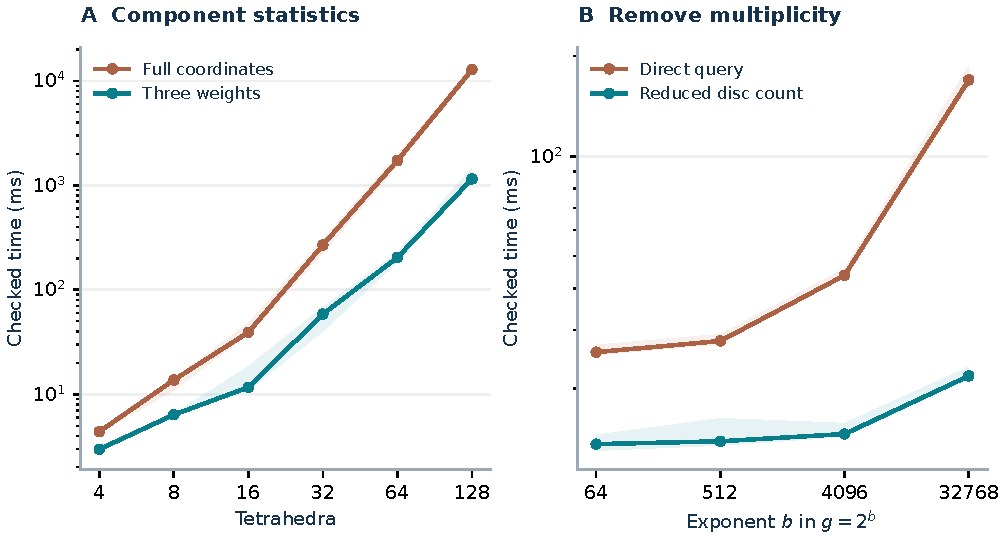
\includegraphics[width=\linewidth]{figures/normal_query_benchmarks.pdf}
\caption{Checked query times from the archived raw samples. Lines show
medians; shaded bands span the observed minimum and maximum of the seven
rounds and are not confidence intervals. Both horizontal axes and the time
axes are logarithmic. Panel A uses supplied normal meridians; panel B uses
the fixed-core family of \cref{tab:core}. No curve is an asymptotic fit.}
\label{fig:normal-benchmarks}
\end{figure}

\subsection{A controlled abstract dimension experiment}

An additional interval-only benchmark holds the endpoint/run structure fixed
while changing the transported dimension. It uses translation and reflection
families, 32-bit and 4,096-bit scales, and dimensions 28, 112 and 448 against
three weights. Its twelve cases have nine arms, nine paired rounds and two
warm-ups per arm. The full checked arm projects and merges its answer to the
same three-coordinate histogram as the compact checked arm. Its paired
ratios range from about 2.0--2.43 at dimension 28 to 18.0--28.34 at dimension
448, with compact A/A ratios 0.935--1.065.

This experiment isolates arithmetic effects more cleanly than the normal
family, where coordinate weights also have more runs. Its dimension parameter
does not describe a triangulation, so these numbers are not normal-surface
or knot-recognition timings. The raw JSON includes smaller-output count-only
controls, producer-only times and replay-only times; none of those smaller
tasks is reported as a same-task speedup over the weighted query. Only the
clean serial run is included in the final evidence.

\section{What would establish quasi-polynomial recognition?}
\label{sec:roadmap}

\subsection{Separate the query bound from the number of queries}

Let $n$ be the size of a knot diagram and suppose a source-bound exterior has
$t=\poly(n)$ tetrahedra. The results above make one supplied-vector disc query
polynomial in $t$ and its coordinate bit length. This remains true if the
normal surface contains exponentially many polygons or components. It gives
no bound on how many candidate vectors a recognizer must try. An exponential
search equipped with a faster polynomial verifier is still an exponential
search.

There are at least two useful directions for continuing the project. A
search-based route can exploit canonical Q-data, certified pruning, and cheap
component predicates. A hierarchy-based route can use the same compressed
primitives when surfaces and their complements are transformed. Neither
direction may replace its missing progress theorem by favorable timings.
The distinction is particularly important for families of layered solid tori:
their exponentially large normal discs stress compressed arithmetic, but the
benchmark hands the disc vector to the algorithm. It does not measure the
difficulty of finding that vector from a knot diagram.

\subsection{A precise conditional budget theorem}

Lackenby's Proposition~9.1 bounds hierarchy iterations by $L(g+1)^L$;
Proposition~10.2 gives $L\le4c_q(\mathcal H_1)$ for the refined process
\cite{Lackenby2026}. The following elementary bookkeeping formulation makes
the desired improvement precise. It is a conditional statement about a
future implementation, not a geometric bound established here.

\begin{proposition}[Sufficient mixed-radix budget]
\label{prop:qp-budget}
Suppose a correct recognition algorithm on an input of size $n$ has a
lexicographically decreasing integer progress vector
$(a_1,\ldots,a_L)$ with $0\le a_i\le G_i$, where the $G_i$ are fixed
nonnegative integers. Suppose these bounds are valid
throughout the entire computation, including suffix reconstruction. Assume
that each phase before the first decrease, between successive decreases,
and after the last decrease performs at most $\poly(n)$ operations,
each costing $\poly(n)$ bit operations on polynomial-size states. If
\[
 L=\poly(n),\qquad
 \sum_{i=1}^{L}\log_2(G_i+1)=O((\log(n+2))^k),
\]
then its running time is
$2^{O((\log(n+2))^{\max(1,k)})}$. In particular, $k=2$ gives
$n^{O(\log n)}$ time.
\end{proposition}
\begin{proof}
Use the mixed-radix integer
\[
 \Phi(a)=\sum_{i=1}^{L}a_i\prod_{j=i+1}^{L}(G_j+1).
\]
It is an integer between zero and $\prod_i(G_i+1)-1$. Decreasing one digit
and replacing any later digits by their largest permitted values still
decreases $\Phi$ by at least one. Thus there are at most
$\prod_i(G_i+1)$ strict decreases. Multiplying this by the polynomial bound
for work between decreases gives
\[
 \log_2 T(n)\le O(\log(n+2))+
                    \sum_i\log_2(G_i+1),
\]
which proves the assertion. The same estimate charges polynomial-size
certificates and their generation and replay whenever they are included in
the per-operation hypothesis.
\end{proof}

Several cautions are mathematically substantive. A linear bound on $L$ and
polynomial bounds on every $G_i$ yield only $2^{O(n\log n)}$ by this argument.
They do not imply quasi-polynomial time. Many digits with $G_i=1$ can already
cause an exponential product. Nor does a logarithmic hierarchy depth help if
the permitted digits have exponential bit lengths. Finally, state-dependent
digit bounds need a single valid potential or a proved amortized replacement;
substituting small bounds observed on one run is insufficient.

The mixed-radix statement identifies a useful research target. One might
bound the total logarithmic digit budget, construct balanced blocks with
certified smaller budgets, or prove that the realizable states occupy a much
smaller set than the entire product box. The last option requires an actual
bound on reachable states and a way to recognize equivalent states within
the intended time. A memoization table without such a theorem can itself
be exponentially large.

\subsection{A compressed transition must preserve its hypotheses}

Polynomial verification and polynomial discovery are different obligations.
Theorem~14.1 of the 2026 hierarchy paper concerns efficient encoding and
checking of an essential hierarchy. Proposition~14.2 supplies a polynomial
compressed transition under its uniform-type, irreducibility and essential
boundary-pattern hypotheses, with a connected normal surface
\cite{Lackenby2026}. The transition caller must establish essentiality for its actual boundary
pattern; a knot-exterior triangulation alone does not supply that hypothesis.

The appropriate implementation objective is consequently a checked transition
whose caller supplies the relevant established hypotheses, or a broader
algorithm with explicit alternative outputs when those hypotheses fail.
Likewise, retaining a small description of the parallelity complement is not
the same as constructing every sheet of the cut-open triangulation. Our
weighted census supplies component data but does not yet retain all attaching
maps required by that transition.

Fast compressed curve operations are relevant to the boundary interface.
For example, Lackenby's curve algorithms compute geometric intersection and
test isotopy in time polynomial in triangulation size and logarithmic curve
weights \cite{LackenbyCurves2026}. Their inputs, essentiality assumptions and
representation changes must be matched explicitly when used for a hierarchy
pattern. The torus homology test in this article is a smaller specialized
operation; the higher-genus obstruction in \cref{sec:geometry} explains why
it cannot replace the more general curve machinery.

\section{A prioritized research agenda}
\label{sec:research-questions}

The next objective is to turn the proved query $x\mapsto\D(x)$ into a
complete recognition procedure with an explicit global complexity bound.
The questions below separate near-term implementation work from structural
estimates that remain to be proved. Throughout, $n$ denotes the crossing
number of the supplied diagram, not the minimum crossing number of its knot.
Each proposed advance should identify its input, its checked output, and the
quantity that decreases or pays for its cost.

\subsection{First priority: certify the diagram-to-exterior construction}

Can the fast diagram pipeline produce a finite triangulation together with
efficiently checkable evidence that it represents the exterior of exactly
the input knot? A useful certificate should describe the local crossing and
arc blocks, their face identifications, and a peripheral marking. Subsequent
simplification should carry a sequence of verified local transformations or
another explicit homeomorphism certificate. The construction must have a
proved polynomial bound on tetrahedra and certificate length in the diagram
encoding.

This bridge makes a positive disc query relevant to the original recognition
problem. The immediate experiment is to attach provenance to existing
diagram-derived fixtures and compare the resulting finite triangulations
with an independent topology implementation. Such comparisons guide
development; the mathematical obligation is a proof for every accepted
construction. Mutation tests should change an arc attachment, a peripheral
label, or a simplification step and require the checker to detect the broken
correspondence.

\subsection{First priority: a complete constrained disc producer}

What search procedure supplies the normal vectors, and how many must it
inspect? The delivered count eliminates a candidate with $\D(x)=0$; it gives
no exhaustion certificate for the remaining admissible vectors. Develop a
producer with a clearly specified finite search space, exact feasibility
bounds, and independently justified pruning rules. Record search nodes,
candidate bit lengths, and time spent in feasibility, lifting, and component
queries separately.

An essential disc can already be found on a Q-vertex ray under the hypotheses
of Suh's theorem; proving that existence again is not the research question
\cite{Suh2010}. The difficult question is whether a complete search can avoid
exponentially many relevant branches on every input. The established
branch-and-bound framework provides a practical comparison
\cite{BurtonOzlen2014}. A proposed pruning rule needs a proof that some
essential-disc witness survives whenever one exists, including when an
intermediate candidate is disconnected or has nonorientable components.

\subsection{First priority: canonicalize before expensive search operations}

Can candidate generation operate directly on primitive quadrilateral data,
constructing the canonical standard lift only when required? Canonical
lifting and vertex-link ambiguity are established Q-theory
\cite{Tollefson1998,Burton2009}. The opportunity is to use them earlier in the
implemented search, so that large common multiplicities and independent
vertex-link offsets never enter its costly orbit queries.

For every proposed Q-coordinate input, construct or certify its integral
lift and check the full admissibility conditions. Evaluate whether branching
bounds can use the coordinate estimate of
Theorem~\ref{thm:primitive-q-core}. The first experiment should compare
search-node and arithmetic counts before and after canonicalization on the
same candidate stream. The identity $\D(x)=g\D(P)$ supports reuse of an
essential-disc count. A request for the original component histogram still
requires its original surface data: vertex-link deletion changes that
histogram, and scaling a one-sided component changes its sheet decomposition.

\subsection{Near-term refinement: certify and benchmark the two-weight mode}

The proposition in \cref{sec:two-weight-refinement} already proves that one
ambient-certified boundary probe suffices for all supplied surfaces in a
fixed supported manifold. Implement its finite binary preprocessing and its
linear-size cocycle witness, then compare two and three weights on identical
candidate streams. The open performance question is the break-even point
between additional ambient preprocessing and the saved transport coordinate.
Cache only source-verified preprocessing data, and include cold and amortized
costs separately. The existing three-weight implementation remains the
reference until the new mode passes the frozen external corpus and the
source-mutation checks. This is an implementation and cost question, not a
conjecture about whether the two-weight criterion is true.

\subsection{Second priority: batch related candidates and reuse checked traces}

How much computation can be shared across candidates in one triangulation?
The canonical core gives an exact starting point: candidates
$x_j=\sum_v\ell_{jv}L_v+g_jP$ share the answer $\D(P)$, with their counts
recovered by multiplication. Cache the validated triangulation, canonical
cores, and their certificates using explicit source identifiers. Charge the
cost of reading each candidate and checking its reduction even on cache hits.

A broader question is whether an interval-orbit trace can be reused over a
region of coordinate space. Equal quadrilateral support alone does not fix
endpoint order or scheduler decisions. A reusable trace would need certified
inequalities and congruences defining where every step remains valid, including
periodic cases. The completed replay artifacts provide a test harness for
this experiment \cite{AHT2006}. Measure reuse per distinct core and per
verified trace region, and retain the total candidate count in the global
cost accounting.

\subsection{Second priority: connect selected components to compressed cutting}

Can a positive three-weight query return enough additional information to
cut along one certified essential disc efficiently? Recover a selected
component's normal vector, using coordinate weights or a targeted orbit
query, and supply the gluing and boundary data needed by the next stage.
This tests a concrete transition from a component predicate to a geometric
operation. A histogram with positive disc multiplicity establishes existence,
but does not by itself specify the cut triangulation.

Compressed cutting must preserve the hypotheses of the routine being used.
Lackenby's hierarchy framework imposes explicit irreducibility and essential
boundary-pattern conditions \cite{Lackenby2026}. Determine how each condition
is established initially and propagated through subsequent cuts, and include
the relevant boundary-pattern evidence in each transition certificate.
Efficient algorithms for curves and normalization offer useful subroutines
\cite{LackenbyCurves2026}; the surrounding three-dimensional invariants still
require proof. Begin with cuts whose outputs have small independent finite
oracles before enlarging the binary weights.

\subsection{Structural priority: prove an amortized hierarchy budget}

Which structural invariant can limit the aggregate search in an accelerated
hierarchy? For a proposed encoding with counters ranging from zero to $g_i$,
a useful \emph{target}, not a theorem established here, is
\[
                 \sum_i\log_2(g_i+1)=O(\log^2 n).
\]
These $g_i$ are hierarchy counter bounds, unrelated to the quadrilateral gcd
of a single input. If all other state choices are charged within the same
budget, the product of the counter ranges is
$2^{O(\log^2 n)}=n^{O(\log n)}$.

The proposed bound must control all reachable states relevant to the
algorithm, including branching and counter resets. A bound along one chosen
successful path is insufficient for an exhaustive search. Seek an invariant
that pays for each split, new boundary pattern, and increase in a counter's
range. The explicit hierarchy machinery in \cite{Lackenby2026} supplies a
precise setting in which to formulate this obligation. Failure to obtain the
target should produce an explicit obstruction family or a weaker proved
budget, rather than an empirical asymptotic claim.

\subsection{Structural priority: anisotropic bounds and a graph of states}

Can individual counter bounds replace a uniform worst-case cap? If an
encoding has $m$ counters, retain $\prod_{i=1}^{m}(g_i+1)$ instead of replacing
it immediately by $(1+\max_i g_i)^m$. This mixed-radix accounting can expose
instances with many small choices and only a few large ones. Identify a
topological reason for that anisotropy and test whether it persists after
cutting and simplification.

Can histories reaching the same certified state be merged into a directed
acyclic graph? State equivalence must preserve the manifold, boundary
pattern, peripheral information, and remaining search obligations. Prove
acyclicity using a well-founded rank, or account explicitly for cycles.
Canonical labels and hashes may locate possible matches, but each merge
needs a verified equivalence. Initial measurements should count distinct
states, transitions, and equivalence-checking cost. A small state graph is
useful only when constructing and recognizing its states is also affordable.

\subsection{Quantitative priority: an explicit deterministic bit bound}

What exponent does the composed algorithm actually satisfy? Derive separate
bounds for triangulation construction, candidate production, integer gcds,
interval operations, weight-run growth, component recovery, cutting, and
certificate checking. Track maximum operand bit lengths and the cost
$M(b)$ of multiplying $b$-bit integers. The weighted AHT theorem gives a
polynomial local foundation \cite{AHT2006}; composition still requires bounds
on the number and size of its invocations.

Publish a deterministic bound with fixed constants, distinguishing
$2^{O((\log n)^2)}$ from $2^{O((\log n)^3)}$ and stating which exponent is
actually proved. Include output and certificate lengths, memory, and input
reading. The completed operation counters and paired kernel measurements
can identify costly terms and check predictions. Their role is to guide
which inequalities need improvement; the final worst-case bound must follow
from the algorithm and its invariants.

\subsection{Continuous priority: stronger adversarial evidence}

Extend the delivered 1,275-vector, 45-triangulation Regina corpus and its
isolated counterexamples. Preserve both essential-disc cancellation and the
orientable sphere-plus-punctured-torus false positive as mandatory cases.
Add large vertex valence, additional boundary vertices, long layered
triangulations, coprime large quadrilateral coordinates, and inputs designed
to increase interval subdivisions. Exercise one-sided scaling and certificate
mutations at every new interface.

Keep a capped corpus with fully expanded independent components and a
separate collection of large binary instances whose answers follow from
proved constructions. For each family, report the parameter varied, the
expected component semantics, the source triangulation, and reproducible
seeds. When recognition stages are connected, add difficult diagram families
and measure every stage on the same instances. This prevents a local speedup
from hiding a newly dominant producer or source-validation cost, while
maintaining the exact distinction between a component of a supplied surface
and a conclusion about the original knot.


\section{Reproduction and repository integration}
\label{sec:reproduction}

\subsection{Archive organization}

The archive contains this PDF, the complete \LaTeX{} source and generated
figures, a portable Python source snapshot, the additive integration patch,
raw audit and benchmark JSON, the frozen external corpus, two explicit
counterexamples, and a manifest of source identities and file hashes.
The top-level \code{README.md} gives the short entry points;
\code{INTEGRATION.md} describes the API contracts and the intended review.
The baseline commit is recorded in full so the work can be compared with
later changes to the repository.

The runnable snapshot is under \code{code/fast}. It preserves the entire
\code{fastunknot} package because the maintained package initializer imports
the existing recognizer infrastructure. Copying only a few local modules
would not preserve ordinary package imports. The snapshot includes only the
selected regression files and the fixture dependencies they require; it does
not carry unrelated historical benchmark directories. The original MIT-0
license and the internal attribution files are retained.

The new functionality consists of six modules: the weighted producer and
independent verifier, the geometric weight construction, the component
census and verifier, and the canonical disc-count wrapper. Two new test files
and four audit or timing drivers accompany them. These additions do not
modify the maintained recognizer's defaults. The integration patch is
intended to be applied at the repository root after checking the pinned
dependency identities; the full snapshot is for reproduction, not an
instruction to overwrite a newer checkout.

\subsection{Commands and optional dependencies}

Python 3.10 or newer is required by the maintained package. The weighted and
native finite-geometry code uses the standard library. Regina is needed for
the external normal-surface audit and the Regina-specific test methods;
those unit methods are reported as skipped if it is absent. Matplotlib is
needed only to regenerate the figures. A \LaTeX{} installation with the
packages named in the main source is needed only to rebuild the PDF.

From the unpacked archive, use:
\begin{quote}\small
\begin{minipage}{\linewidth}
\begin{verbatim}
python3 reproduce.py tests
python3 reproduce.py audit
python3 reproduce.py regina
python3 reproduce.py benchmark
python3 reproduce.py figures
python3 reproduce.py paper
python3 reproduce.py verify-manifest
\end{verbatim}
\end{minipage}
\end{quote}

The benchmark command runs the recorded full experiment sizes, so it takes
longer than the finite audits. The launcher uses the current Python
interpreter and supplies the import paths explicitly. Recomputed results go
to \code{reproduced/}, preserving the archived measurements in
\code{results/}. The Regina command reads the frozen corpus instead of
reenumerating vertex solutions, reducing sensitivity to enumeration order
in another Regina release. The generator can also construct a new corpus
when that is the intended experiment.

Tables and plots are generated from raw results by
\code{article/make_figures.py}; the corresponding CSV is included. A paper
rebuild uses the archived figures and tables unless they are explicitly
regenerated. The main \LaTeX{} file uses a self-contained bibliography, so
BibTeX is unnecessary. The manifest check compares bytes; it does not claim
that independently rerun timing JSON or PDF timestamps must match byte for
byte.

\subsection{Minimal native use}

The following example runs entirely on the included finite fixture. Its
expected count is two even though the total boundary class is zero.
\begin{quote}\small
\begin{minipage}{\linewidth}
\begin{verbatim}
from normal_orbit_research.fixtures import layered_torus
from fastunknot.normal_surface_components import normal_component_census
from fastunknot.normal_component_verify import (
    verify_normal_component_certificate,
)

tri, meridian = layered_torus(4)
vector = [[2 * value for value in row] for row in meridian]
answer = normal_component_census(tri, vector,
                                 record_certificate=True)
assert answer['compressing_disk_components'] == 2
assert verify_normal_component_certificate(
    tri, vector, answer['certificate'])
\end{verbatim}
\end{minipage}
\end{quote}

The separate executable example also creates a large input with coordinate
gcd one, verifies its canonical reduction, and saves both proof objects.
This gives an integration reviewer an immediately inspectable positive case,
an independent replay path, and explicit evidence of the source contract.

\subsection{Acceptance criteria for the next integration}

A reasonable first merge criterion is preservation of the old normal and
interval APIs, successful replay of the saved corpus, rejection of the
recorded source and histogram forgeries, and a caller-facing distinction
between a complete query and an inconclusive work limit. A later recognizer
integration should additionally specify the provenance witness and the
candidate-generation contract before using a positive disc count as a knot
decision. The benchmark scripts should remain usable as those later stages
are introduced, with separate measurements for discovery, transport,
reconstruction and verification.

The concrete result available now is a compressed, checked operation that
was missing from the native backend, together with a smaller exact input
for its essential-disc count. The next mathematical milestone is a bound on
the complete search or hierarchy that calls such operations, with every
representation change and bit cost charged.

\begin{thebibliography}{99}
\small\raggedright
\addcontentsline{toc}{section}{References}

\bibitem{AHT2006}
I.~Agol, J.~Hass, and W.~Thurston,
\emph{The computational complexity of knot genus and spanning area},
Transactions of the American Mathematical Society \textbf{358} (2006),
3821--3850.
\url{https://arxiv.org/html/math/0205057v2}.
In particular, Theorems~12 and~16 and Corollary~17.

\bibitem{Tollefson1998}
J.~L.~Tollefson, \emph{Normal surface Q-theory},
Pacific Journal of Mathematics \textbf{183}(2) (1998), 359--374.
\url{https://doi.org/10.2140/pjm.1998.183.359}.

\bibitem{Burton2009}
B.~A.~Burton,
\emph{Converting between quadrilateral and standard solution sets in normal
surface theory}, Algebraic \& Geometric Topology \textbf{9}(4) (2009),
2121--2174.
\url{https://doi.org/10.2140/agt.2009.9.2121};
\url{https://arxiv.org/html/0901.2629v2}.
In particular, Lemma~2.5, Definition~3.9 and Lemma~3.11.

\bibitem{Suh2010}
C.-H.~Suh, \emph{The unknotting problem and normal surface Q-theory},
preprint (2010), arXiv:1009.1500.
\url{https://arxiv.org/abs/1009.1500}.

\bibitem{BurtonOzlen2014}
B.~A.~Burton and M.~Ozlen,
\emph{A fast branching algorithm for unknot recognition with experimental
polynomial-time behaviour}, preprint, arXiv:1211.1079v3 (2014;
originally posted 2012).
\url{https://arxiv.org/html/1211.1079v3}.

\bibitem{LackenbySlides}
M.~Lackenby, \emph{The unknot recognition problem},
Oxford talk slides, March 2021, particularly the displayed
$2^{O((\log n)^3)}$ bound.
\url{https://people.maths.ox.ac.uk/lackenby/quasipolynomial-talk-oxford.pdf}.

\bibitem{Oxford2021}
Mathematical Institute, University of Oxford,
\emph{Marc Lackenby announces a new unknot recognition algorithm that
runs in quasi-polynomial time}, institutional research announcement,
2 February 2021.
\url{https://www.maths.ox.ac.uk/node/38304}.

\bibitem{Lackenby2026}
M.~Lackenby, \emph{Incompressible surfaces, hierarchies and unknot recognition},
preprint, arXiv:2607.23350v1, 25 July 2026.
\url{https://arxiv.org/html/2607.23350v1}.

\bibitem{LackenbyCurves2026}
M.~Lackenby, \emph{Some fast algorithms for curves in surfaces},
Discrete \& Computational Geometry \textbf{76} (2026), 539--588.
\url{https://doi.org/10.1007/s00454-026-00845-7}.
Author text consulted:
\url{https://people.maths.ox.ac.uk/lackenby/AlgorithmsSurfaces13jan26.pdf}.

\bibitem{Regina}
B.~A.~Burton, R.~Budney, W.~Pettersson, et al.,
\emph{Regina: Software for low-dimensional topology}, 1999--2025.
\url{https://regina-normal.github.io/}.
The audit used Python package 7.4.1 (engine reports version 7.4).

\bibitem{Hatcher2002}
A.~Hatcher, \emph{Algebraic topology}, Cambridge University Press, 2002.
Section~3.3, in particular Theorem~3.43 (duality for manifolds with boundary).
\url{https://pi.math.cornell.edu/~hatcher/AT/AT.pdf}.

\bibitem{ProveItSnapshot}
V.~Reshetnikov and ProveIt contributors,
\emph{ProveIt: Topology/UnknotRecognition}, source snapshot
\texttt{7518823550fbc8c217bc8be0113fe52002e77465},
9 October 2026 UTC.
\url{https://github.com/VladimirReshetnikov/ProveIt/tree/7518823550fbc8c217bc8be0113fe52002e77465/Topology/UnknotRecognition}.
The accompanying manifest identifies unchanged baseline dependencies and
the additive continuation files.

\end{thebibliography}

\end{document}
